\chapter{Introduction}
\label{chp:introduction}
\section{Motivation}
\label{sec:motivation}
The European Union (EU) has pledged to cut the consumption of primary energy by 20\%, by the year 2020.  It is estimated that buildings consume 40\% of the energy produced\footnote{according to value published at https://ec.europa.eu/energy/en/topics/energy-efficiency/buildings }.  This has resulted in an increase in the demand to reduce the energy consumption of buildings. To reduce the consumption of energy, building automation systems (BAS) are being widely employed. BAS are computer-based systems that help to manage, control and monitor building technical services (HVAC, lighting etc.) and the energy consumption of devices used by the building. It is estimated that BAS can save a building between 5 \% to 30 \% on the utility cost by managing HVAC and lighting systems\cite{bas}. Figure \ref{fig:BAS} illustrates a building equipped with BAS.

\begin{figure}[!ht]
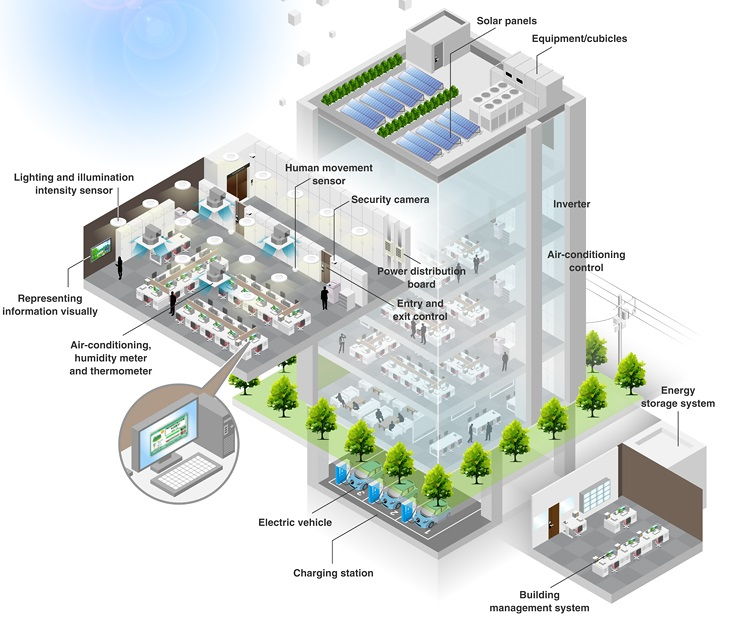
\includegraphics[width=\textwidth]{./pics/bms.jpg}
\caption{Illustration of a building equipped with BAS.}
\label{fig:BAS}
\end{figure}

BAS deploy a huge number of sensors, which provide inputs to perform efficient control of various services. BAS brings with it various benefits, and at the same time offers numerous challenges too. For BAS, sensor measurements alone are not sufficient to understand the condition of the facilities, unless combined with meta-data associated with the sensors.
Meta-data as defined in \cite{gao2015data} refers to any information associated  with the device that helps to contextualize the measurements or control signals regularly being sent from/to the device, such as the location within the building, the physical phenomenon being sensed, etc. One of the major challenges in a BAS system is generating and updating the meta-data of the sensors while they are deployed or replaced.
One of the important meta-data required is that of the physical location of the sensor as discussed in \cite{liu2009requirements}.
As the size and distribution of the deployed sensors are high, it is highly cumbersome and error prone to manually maintain the meta-data about the sensor placement. Apart from being error prone, the manual configuration has to be repeated every time there is a change in the meta-data. Change in meta-data can be due to various reasons, such as a change in the office setup, replacement and/or relocation of sensors. All these factors result in inaccurate information about the location of the sensors. Without accurate information of the location of the sensors, interpreting the data collected from the sensor is difficult and also can be misleading. This could result in the decrease in the effectiveness of the deployed BAS systems. Hence there is a need to develop methods to accurately determine the location of the sensors within the building.
\section{System Description}
Smart lighting control is one of the major components of BAS. Lighting is responsible for 11\%  and 18\% of the energy consumption in case of residential and commercial buildings respectively\cite{website}. 
State of the art lighting control employs co-located occupancy sensors and light sensors, placed on luminaires which are attached to the ceiling\cite{pandharipande2015smart,caicedo2016smart,van2014distributed}. Figure \ref{fig:sysDes} shows an illustration of one such system. In this thesis, we consider a centrally controlled lighting systems with such ceiling mounted sensor grid. Occupancy sensors provide information about the occupancy of the space and the light sensors measure the intensity of the light within the field of view of the sensors. A centrally located controller using this information from the sensors, controls the lights so as to ensure that the space is lit to a suitable intensity level.

In this thesis, we make use of only the occupancy sensors, whose output is binary. 
We use the notation $1$ representing occupancy and $0$ representing an unoccupied space, within the sensors field of view. 
We represent the sensors grid as a graph $G$ with the sensors located on the vertices of the graph. We assume that the Cartesian coordinates, either relative or absolute of the vertices of the grid are available. 

\begin{figure}[!ht]
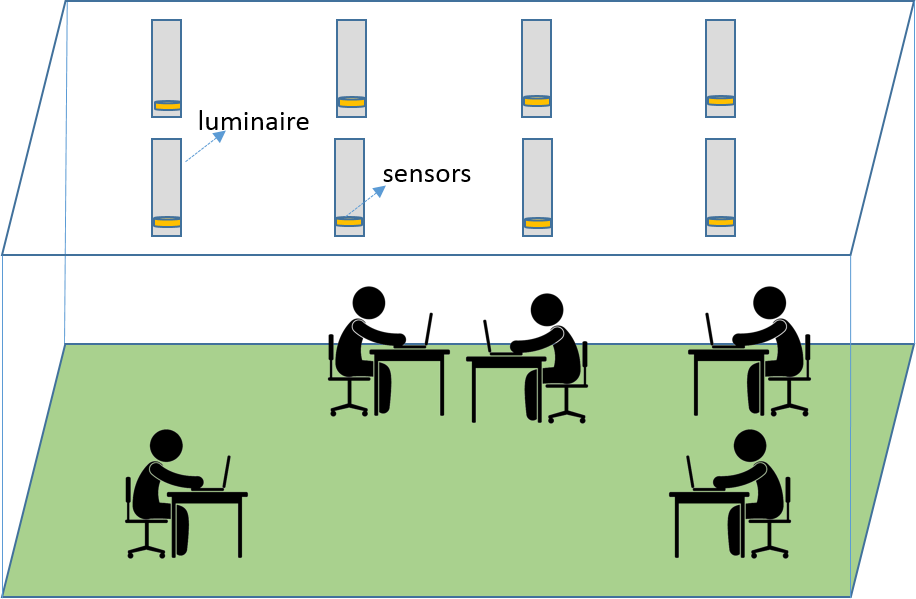
\includegraphics[scale=0.75]{./pics/systemDescription.png}
\caption{Illustration of smart indoor lighting system with co-located sensors}
\label{fig:sysDes}
\centering
\end{figure}

\section{Problem Statement}

Several studies  have been carried out to infer the sensor location from sensor data \cite{Hong:2013:TAS:2528282.2528302,doi:10.1061/9780784413616.226,Koc:2014:CLC:2674061.2674075,Lu:2014:SBS:2648771.2629441,ellis2012creating,muller2014automated,marinakis2005learning}. Most of the methods developed so far have identified ways to cluster the sensors that are located within their proximity; however the methods do not identify where exactly on the grid each sensor is located in a dense sensor grid \cite{Hong:2013:TAS:2528282.2528302,doi:10.1061/9780784413616.226,Koc:2014:CLC:2674061.2674075}.  Therefore the research question that is being tackled in this work is:

\textit{How to automatically determine the location of the sensors utilizing binary data from the ceiling mounted occupancy sensors and the information about the grid (coordinates of the vertices constituting the grid)?}\\



The major challenges in solving the problem are:
\begin{itemize}
\item In a data driven localization method, the first step is identifying the neighbors of a sensor.
By neighbors, we refer to all the sensors which have an overlapping field of view with the sensor under consideration.
As described earlier we consider binary occupancy sensors in our system.
Since in the overlapping region the neighboring sensors observe the same event, these sensors will be triggered simultaneously.
Hence a straightforward way of identifying the neighboring sensors would be to look for sensors where simultaneous triggers are observed.
But when multiple people are present in the space under consideration, simultaneous triggers can be observed even for non neighboring sensors. 
This makes it difficult to distinguish between the neighboring and non-neighboring sensors.
Also, raw data from the sensors do not provide any extra information about the occupant or the activity that is happening in the space, the challenge is to identify a feature that can be extracted from the sensor's data that will help in differentiating neighboring and non neighboring sensors.
\item After identifying sensors within each other's neighborhood, deriving the location information utilizing the grid information is non trivial. 
There are several possible ways in which these cluster of neighboring sensors can be arranged on the grid. 
Out of these several possible ways, the challenge is to identify the true arrangement of the sensors on the grid.
\end{itemize}


\section{Contributions of the thesis}
The main contributions of the thesis are:
\begin{itemize}
\item Use of energy feature of the binary occupancy sensor data to distinguish between neighboring and non-neighboring nodes.\par
From binary occupancy sensor data, we compute the energy feature using a moving window with 50\% overlap.
We determine the window length empirically. 
We use this energy feature to calculate the correlation between the sensors.
 Using these correlation values in this work we develop a method to distinguish between the neighboring and non-neighboring nodes.
\item Determine a criteria to obtain the true arrangements of the sensor with the help of correlation coefficients between the sensors.\par
Given $n$ sensors, these sensors can be arranged on the grid in $n!$ ways. Using the correlation values between the sensors we define a quantity called Grid Correlation Sum (GCS), which is used to identify the precise arrangement of the sensors on the grid.
\item Establish a relationship between the correlation coefficients among the sensors and the sensor grid.\par
In this thesis, we show that there exists a relationship between the maximum spanning tree (MST) obtained from the correlation coefficient between all the sensors and the sensor grid. We show that the MST represents one of the spanning trees for the sensor grid.
\item Reducing the problem of determination of sensor locations  on the grid to a problem of graph matching \cite{conte2004thirty}.\par
 Using the relationship established between the MST of correlation coefficients and the sensor grid, we use graph matching technique to obtain the various mapping between the sensors and the grid vertices. Out of the various mapping obtained using $GCS$ we determine the actual mapping  between the sensor nodes and the grid vertices.
\end{itemize}

\section{Outline of thesis}

The rest of the thesis is organized as follows: in Chapter \ref{chp:litReview}, we give a brief overview of related work. In Chapter \ref{chp:method}, we present the method that has been developed. In Chapter \ref{chp:testbed}, we describe our testbed setup. Next, in Chapter \ref{chp:res}, we present the results obtained by applying the method that we have developed on actual sensor data obtained rom 2 different testbeds. In the end in Chapter \ref{chp:conclusionsandfuturework}, we conclude the work done and discuss future work.




